% latex table generated in R 3.6.3 by xtable 1.8-4 package
% Tue Jan 16 13:09:39 2024
\begin{table}[ht]
\centering
\begin{tabular}{rlrrr}
  \hline
 & OTU & MeanRA & MedianRA & SE \\ 
  \hline
1479019 & Methylobacterium sp. C & 0.00007633 & 0.00007547 & 0.00000216 \\ 
  299262 & Tateyamaria omphali & 0.00010673 & 0.00010456 & 0.00000349 \\ 
  1858609 & Acidovorax sp. T & 0.00011493 & 0.00010232 & 0.00000968 \\ 
  1658672 & Ottowia sp. oral taxon 89 & 0.00013825 & 0.00013775 & 0.00000374 \\ 
  2202141 & Chromobacterium phragmiti & 0.00011981 & 0.00011471 & 0.00000336 \\ 
  658630 & Pseudomonas sp. CMR5 & 0.00008522 & 0.00007885 & 0.00000672 \\ 
  1881017 & Pseudomonas sp. 7SR & 0.00008174 & 0.00006956 & 0.00000750 \\ 
  2054919 & Pseudomonas sp. S09G 35 & 0.00004755 & 0.00004597 & 0.00000304 \\ 
  2774873 & Pseudomonas sp. ADP & 0.00005952 & 0.00004786 & 0.00000683 \\ 
  2219057 & Pseudomonas sp. LG1E & 0.00003061 & 0.00002850 & 0.00000180 \\ 
  1898684 & Pseudomonas sp. LPH & 0.00004548 & 0.00002501 & 0.00001203 \\ 
  2590776 & Pseudomonas sp. NIBRBAC00050277 & 0.00002328 & 0.00002083 & 0.00000190 \\ 
  2774459 & Pseudomonas sp. IzPS5 & 0.00002884 & 0.00002700 & 0.00000225 \\ 
  200450 & Pseudomonas triviali & 0.00007870 & 0.00007535 & 0.00000487 \\ 
  183795 & Pseudomonas mediterrane & 0.00006965 & 0.00005698 & 0.00000853 \\ 
  29442 & Pseudomonas tolaasi & 0.00004854 & 0.00004475 & 0.00000300 \\ 
  75588 & Pseudomonas libanensi & 0.00002296 & 0.00001980 & 0.00000186 \\ 
  1691904 & Pseudomonas sedimini & 0.00007117 & 0.00004577 & 0.00001392 \\ 
  1853130 & Pseudomonas silesiensi & 0.00005116 & 0.00004823 & 0.00000342 \\ 
  1434072 & Halopseudomonas salegen & 0.00005960 & 0.00005114 & 0.00000621 \\ 
  1073999 & Cronobacter condimenti & 0.00002925 & 0.00002816 & 0.00000115 \\ 
  2666185 & Spiribacter sp. 243 & 0.00011615 & 0.00011621 & 0.00000390 \\ 
  2661612 & Pseudodesulfovibrio & 0.00004334 & 0.00004365 & 0.00000183 \\ 
  1894 & Kitasatospora aureofacien & 0.00007564 & 0.00007907 & 0.00000520 \\ 
  300019 & Microbacterium paludicol & 0.00003330 & 0.00002934 & 0.00000293 \\ 
  256701 & Glutamicibacter arilaitensi & 0.00004168 & 0.00004316 & 0.00000315 \\ 
  1630135 & Dermabacter vaginali & 0.00007216 & 0.00007167 & 0.00000313 \\ 
  83262 & Mycobacteroides immunogenu & 0.00011016 & 0.00010334 & 0.00000493 \\ 
  441500 & Corynebacterium timonens & 0.00009727 & 0.00009133 & 0.00000364 \\ 
  43771 & Corynebacterium urealyticu & 0.00006312 & 0.00006273 & 0.00000245 \\ 
  43770 & Corynebacterium striatu & 0.00004302 & 0.00004224 & 0.00000233 \\ 
  203263 & Corynebacterium aquila & 0.00003411 & 0.00003577 & 0.00000180 \\ 
  2609299 & Actinobaculum & 0.00004557 & 0.00004722 & 0.00000257 \\ 
  35760 & Bifidobacterium choerinu & 0.00011989 & 0.00012381 & 0.00000479 \\ 
  1335613 & Gordonibacter urolithinfacien & 0.00009591 & 0.00009744 & 0.00000181 \\ 
  604330 & Parafannyhessea umbonat & 0.00011704 & 0.00011906 & 0.00000404 \\ 
  1871022 & Parolsenella massiliensi & 0.00007758 & 0.00007810 & 0.00000239 \\ 
  365617 & Paenibacillus sabina & 0.00004839 & 0.00004879 & 0.00000176 \\ 
  2610894 & Flintibacter & 0.00004748 & 0.00004828 & 0.00000247 \\ 
  2614128 & Clostridium & 0.00005019 & 0.00004795 & 0.00000247 \\ 
  42837 &   & 0.00007226 & 0.00007016 & 0.00000298 \\ 
  92942 & Nostoc lincki & 0.00002378 & 0.00001464 & 0.00000550 \\ 
  2618749 & Scytonema & 0.00008482 & 0.00008961 & 0.00000847 \\ 
  980427 & Deinococcus wulumuqiensi & 0.00014906 & 0.00014494 & 0.00000394 \\ 
  1299 & Deinococcus radioduran & 0.00012662 & 0.00012342 & 0.00000325 \\ 
  310783 & Deinococcus desert & 0.00009394 & 0.00009060 & 0.00000429 \\ 
  454171 & Chthonomonas calidirose & 0.00007864 & 0.00007652 & 0.00000248 \\ 
  290174 &   & 0.00001626 & 0.00001591 & 0.00000115 \\ 
  869211 & Spirochaeta thermophila & 0.00002979 & 0.00002963 & 0.00000142 \\ 
  62320 & Haloterrigena turkmenic & 0.00008121 & 0.00008087 & 0.00000363 \\ 
  370324 & Natrinema longu & 0.00005274 & 0.00005464 & 0.00000214 \\ 
  13769 & Natrialba magadi & 0.00007369 & 0.00007005 & 0.00000315 \\ 
  1175445 & Methanocella arvoryza & 0.00003724 & 0.00003540 & 0.00000206 \\ 
  1826872 & Candidatus Nitrosocosmicus hydrocol & 0.00007780 & 0.00005223 & 0.00001720 \\ 
   \hline
\end{tabular}
\caption{Keystone OTUs of } 
\end{table}
\begin{figure}
\centering
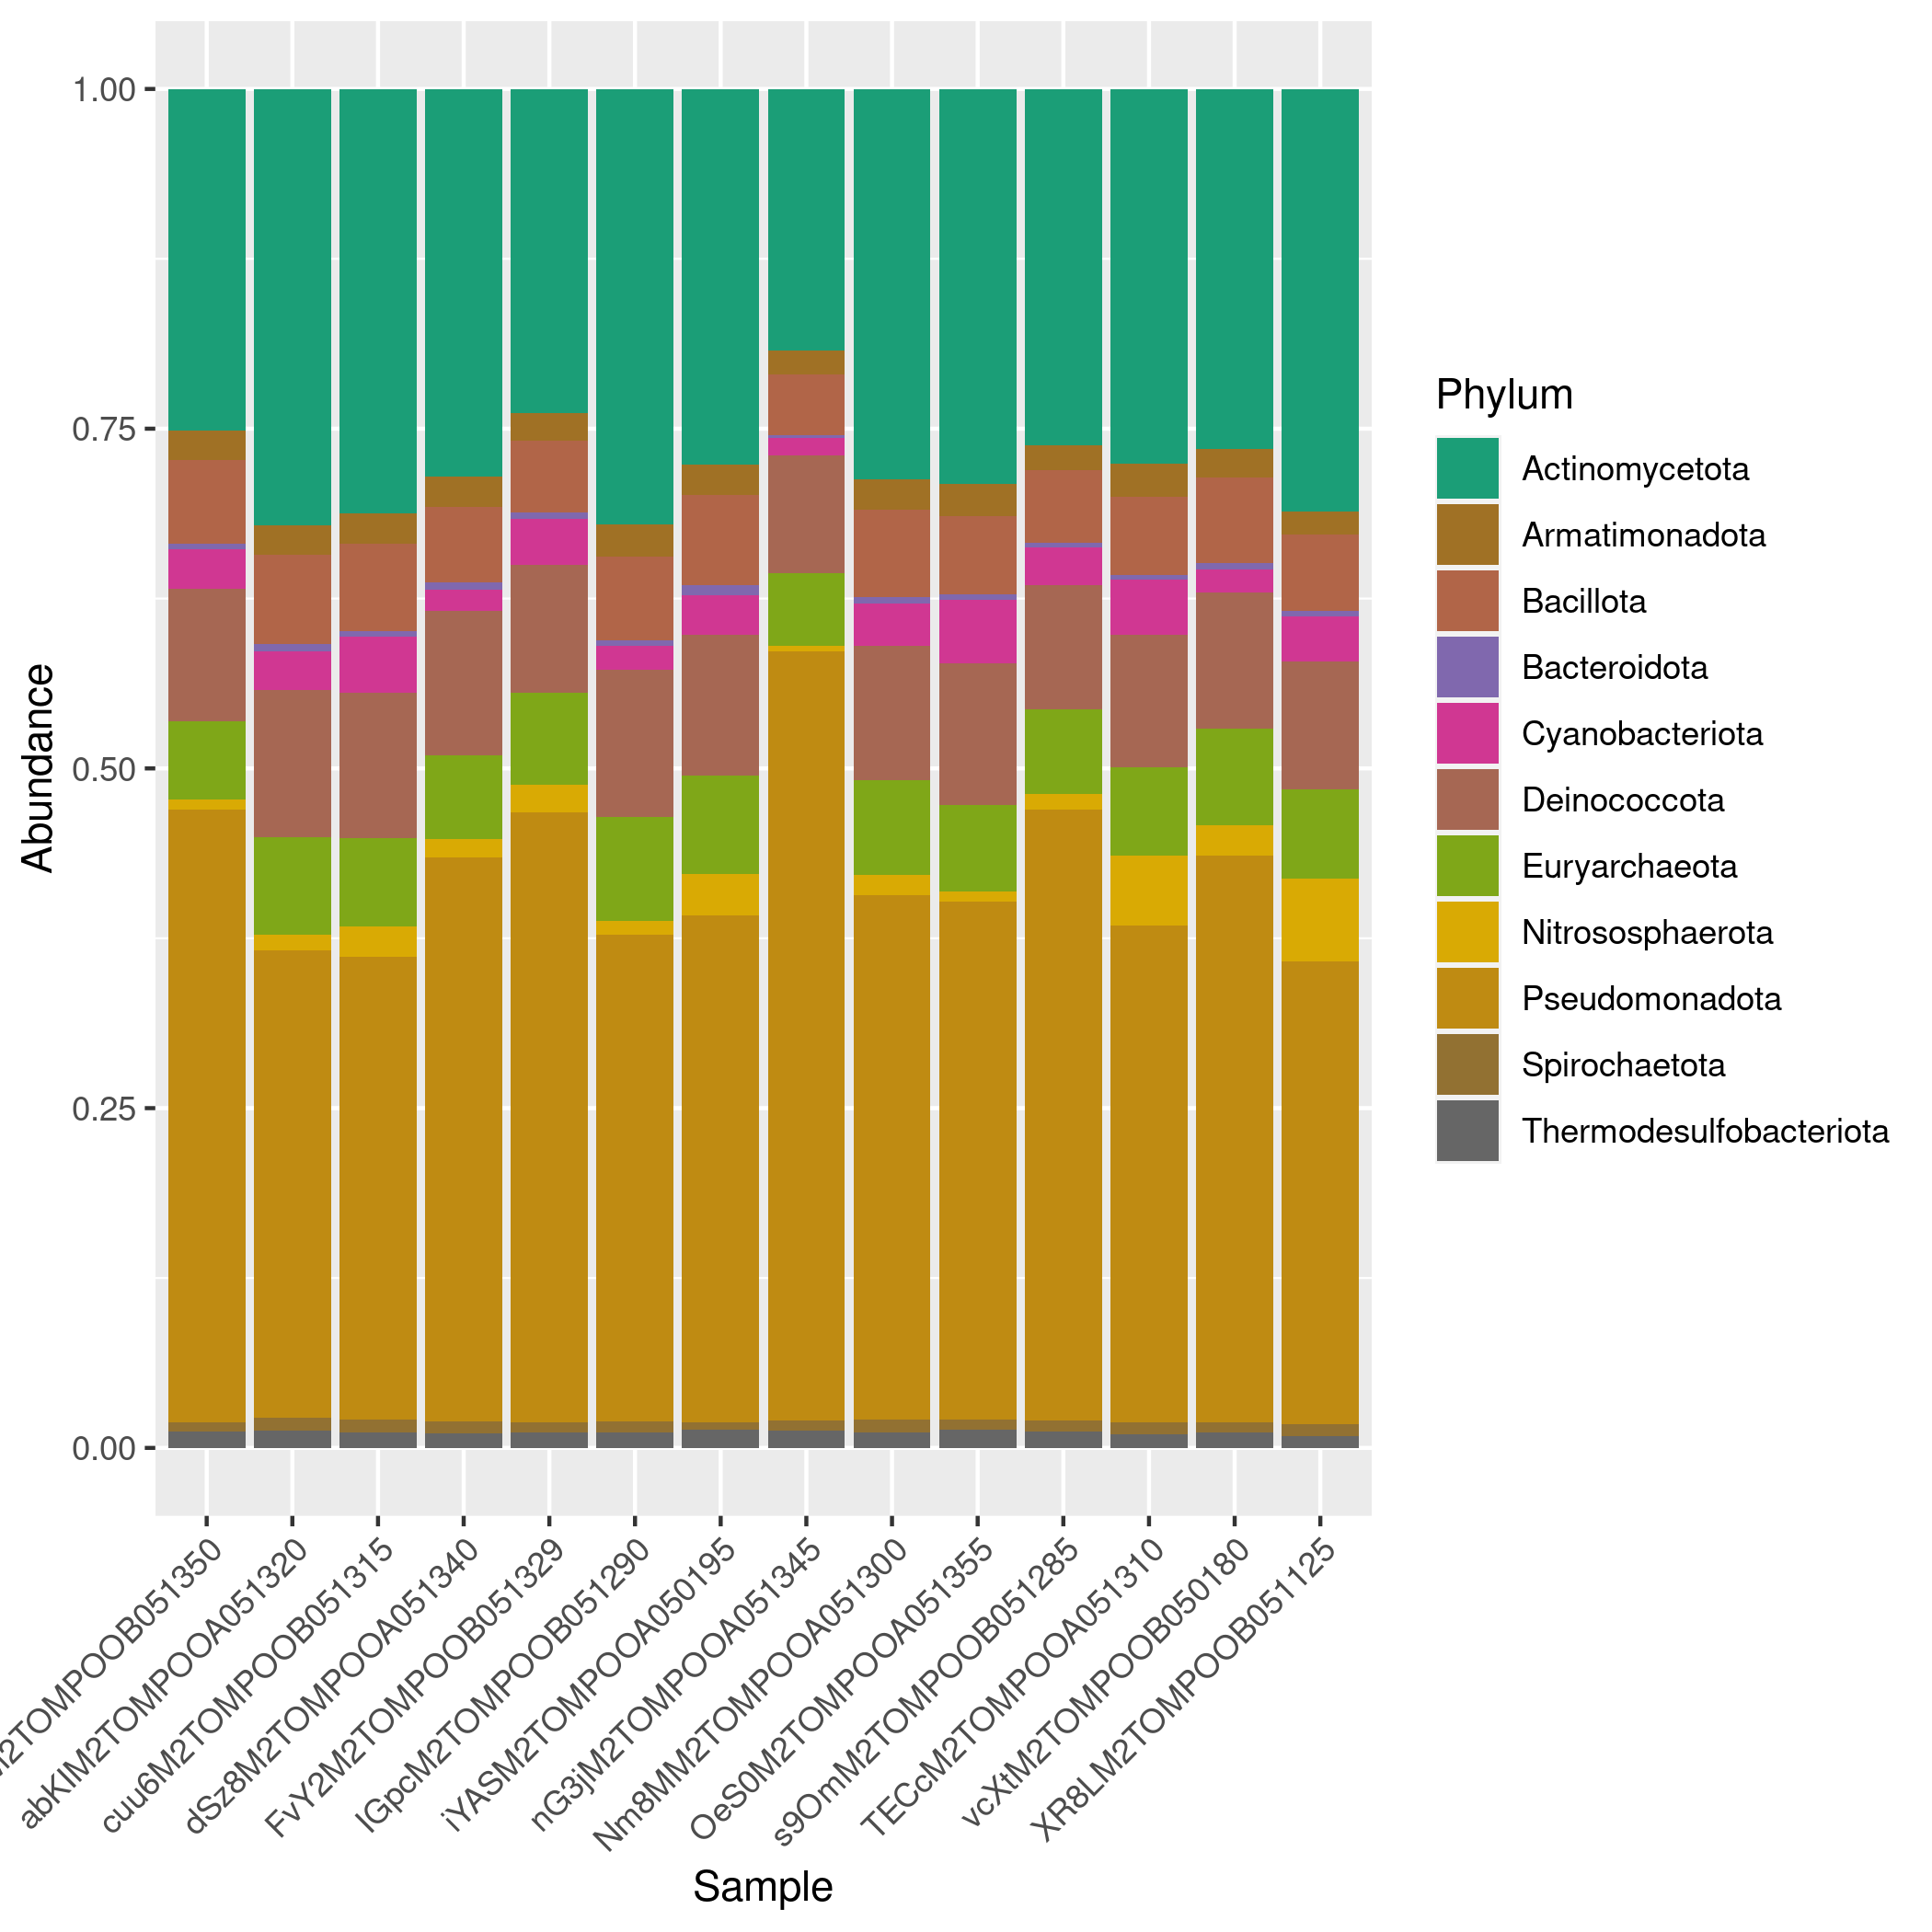
\includegraphics[scale = 0.8]{tomate_desarrollo.csv_relative_abundance_Phylum.png}
\caption{Relative abundance by phyla of keystone OTUs }
\label{fig:tomate_desarrollo.csv_phyla}
\end{figure}
\begin{figure}
\centering
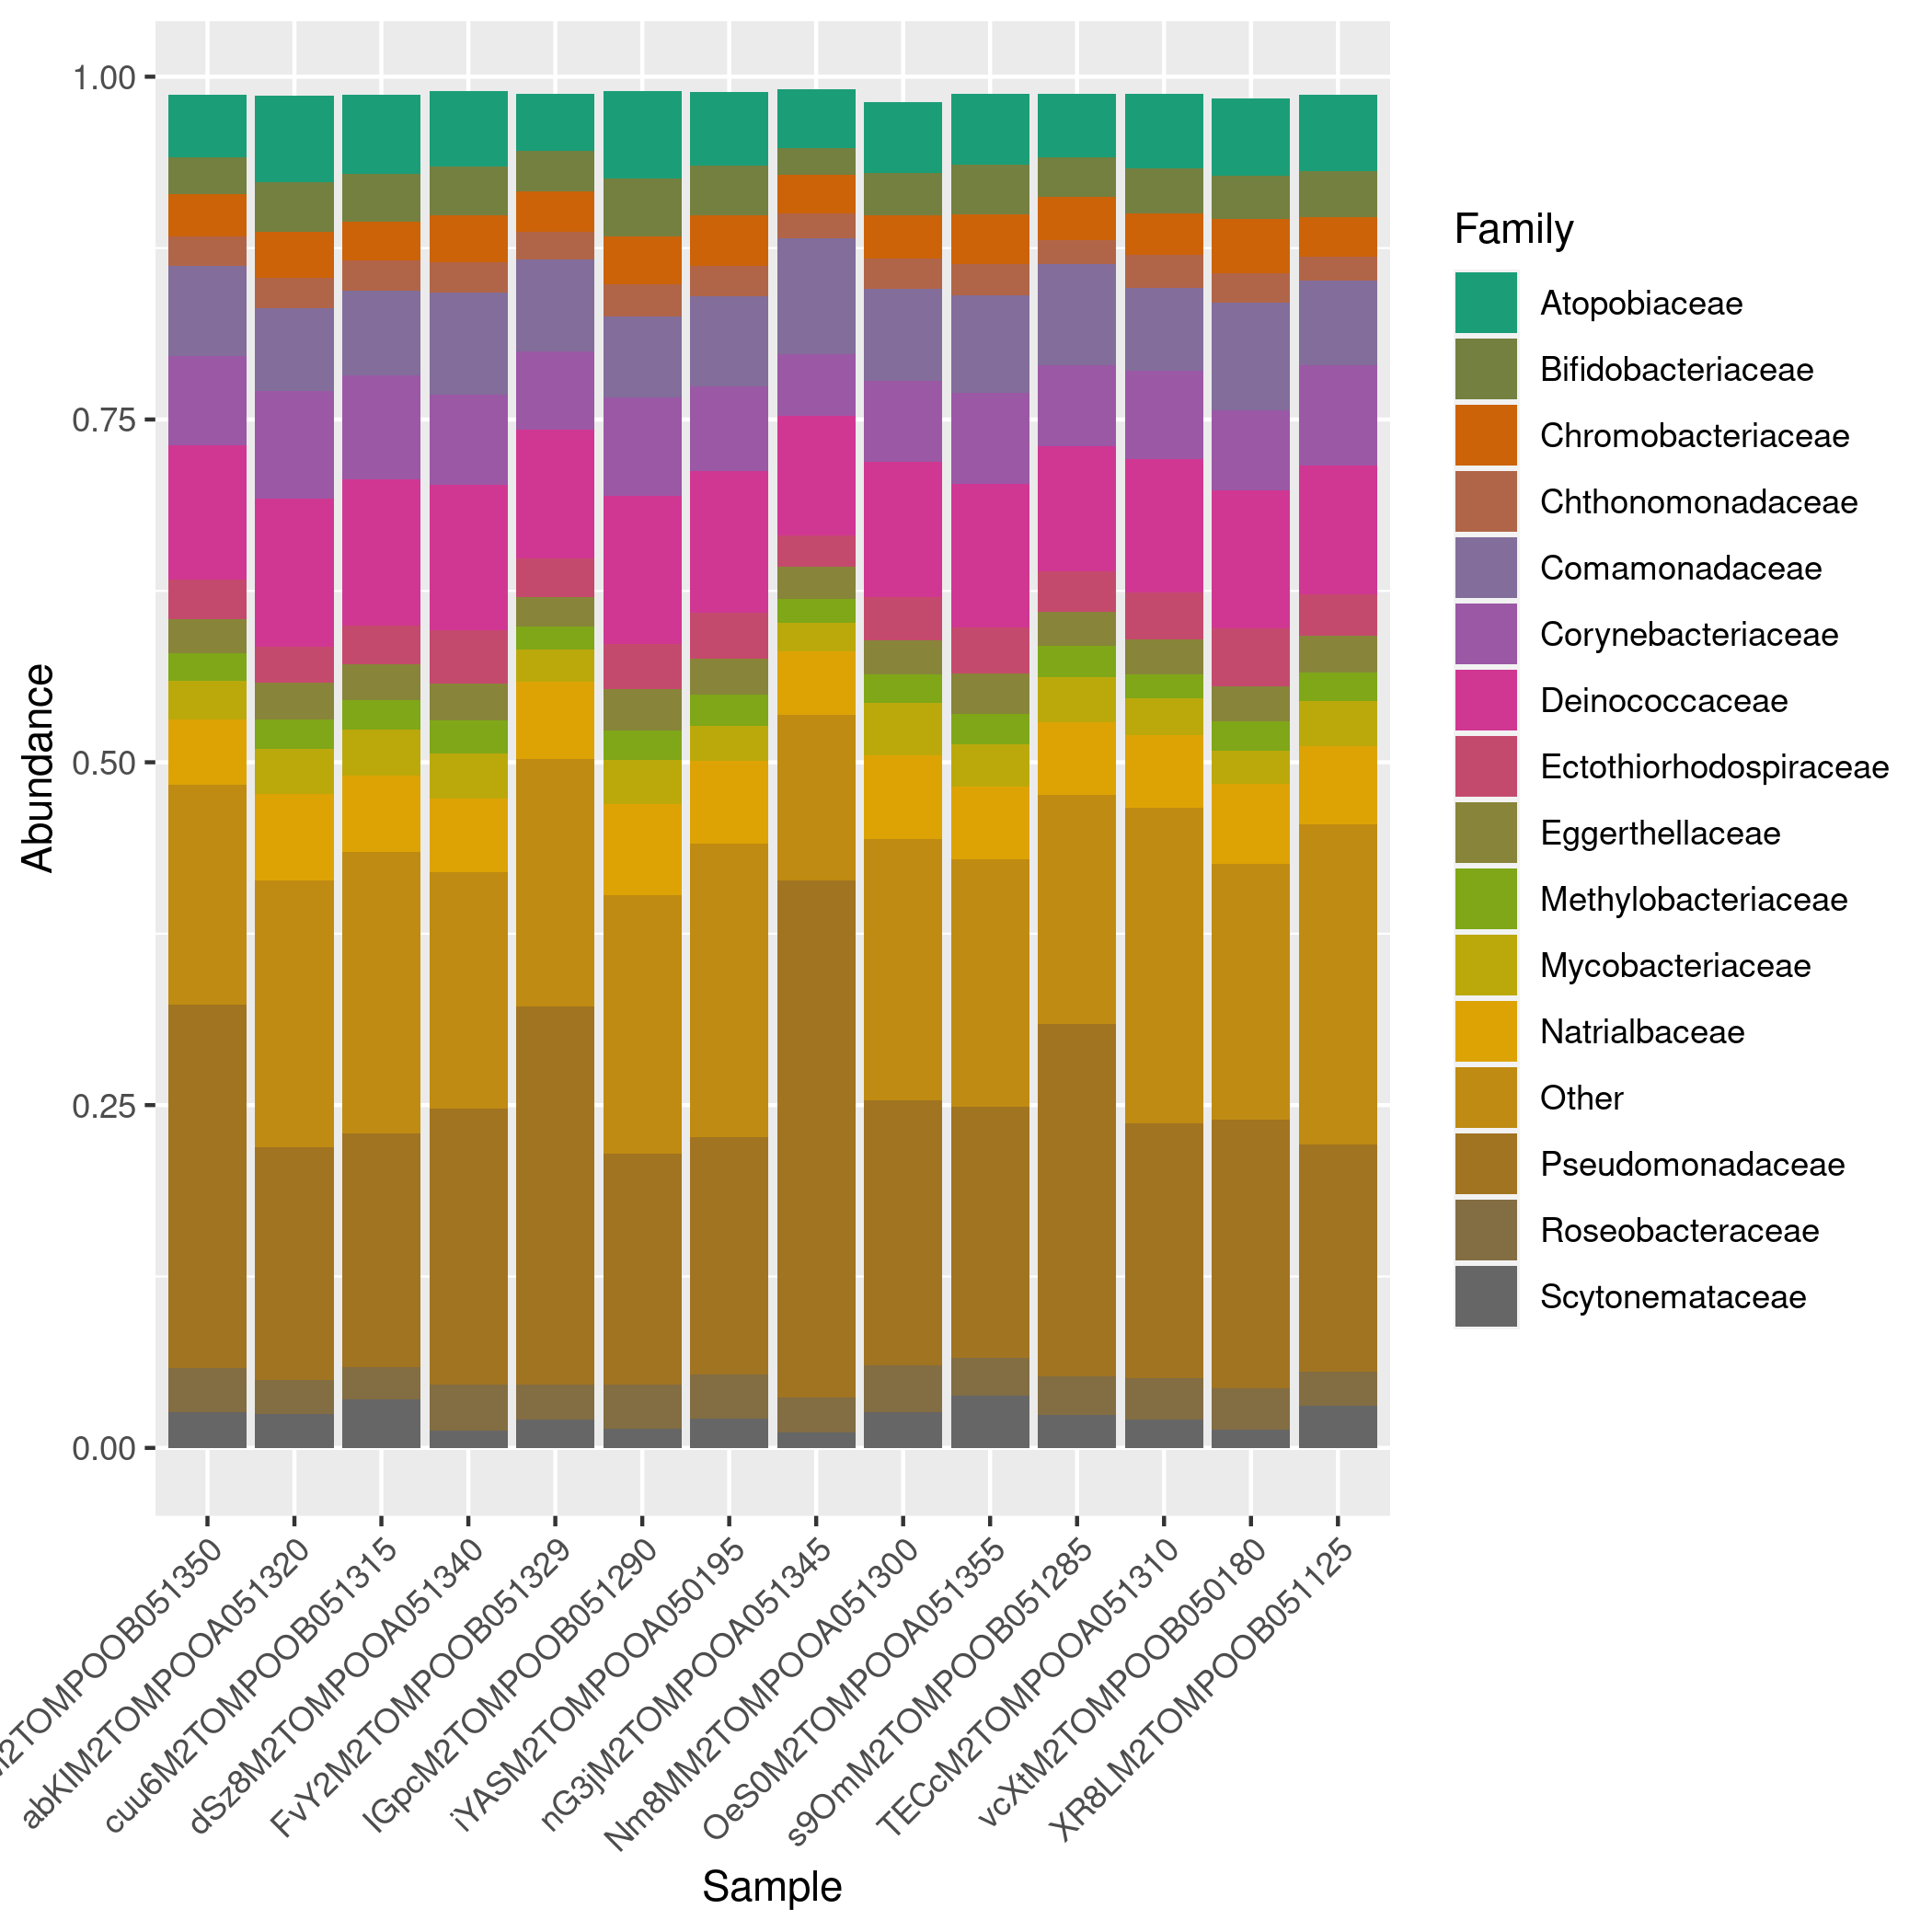
\includegraphics[scale = 0.8]{tomate_desarrollo.csv_relative_abundance_Family.png}
\caption{Relative abundance by families of keystone OTUs }
\label{fig:tomate_desarrollo.csv_family}
\end{figure}
\begin{figure}
\centering
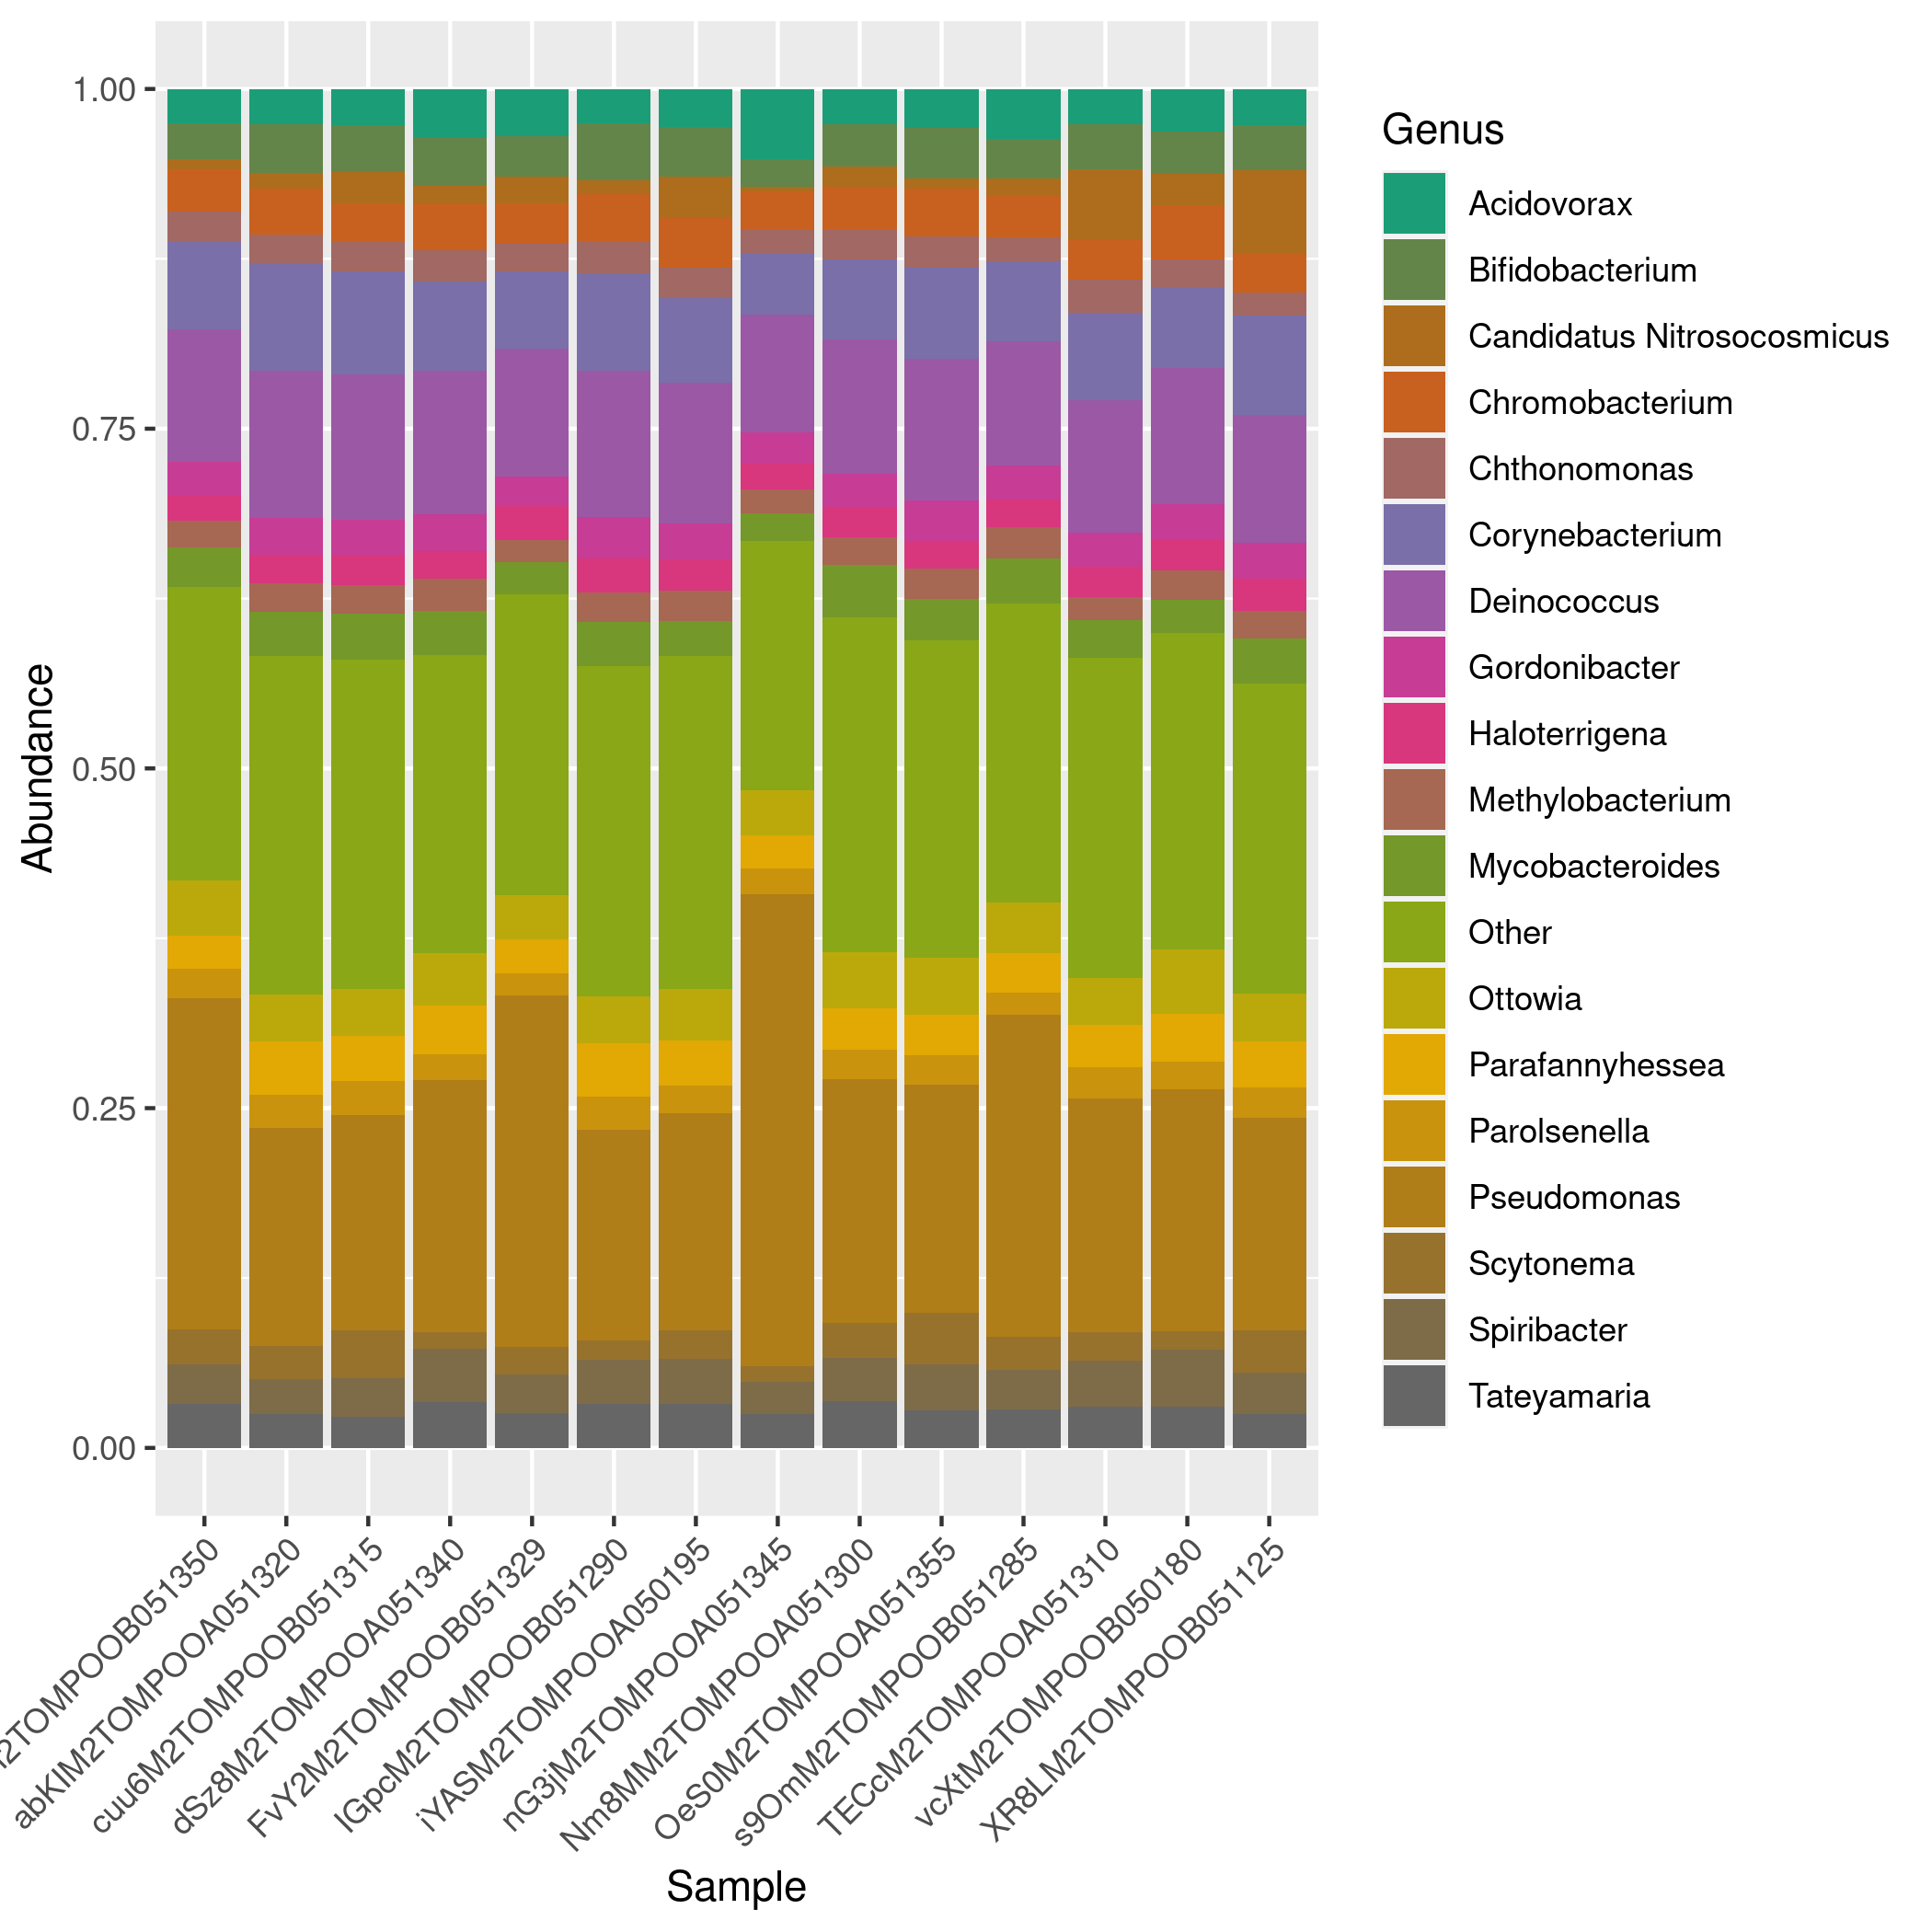
\includegraphics[scale = 0.8]{tomate_desarrollo.csv_relative_abundance_Genus.png}
\caption{Relative abundance by genera of keystone OTUs }
\label{fig:tomate_desarrollo.csv_genus}
\end{figure}
